\subsection{Rimbalzi}

Guardando l'istogramma 2D delle misure in coincidenza, abbiamo notato dei comportamenti non attesi che abbiamo supposto e poi verificato essere dei fotoni che rimbalzano da un rivelatore all'altro.

La \autoref{scatter} mostra un tipico istogramma 2D
nella configurazione in cui 2 rivelatori sono posti uno di fronte all'altro alla stessa distanza da una sorgente di \na{}.

\begin{figure}[h]
\centering
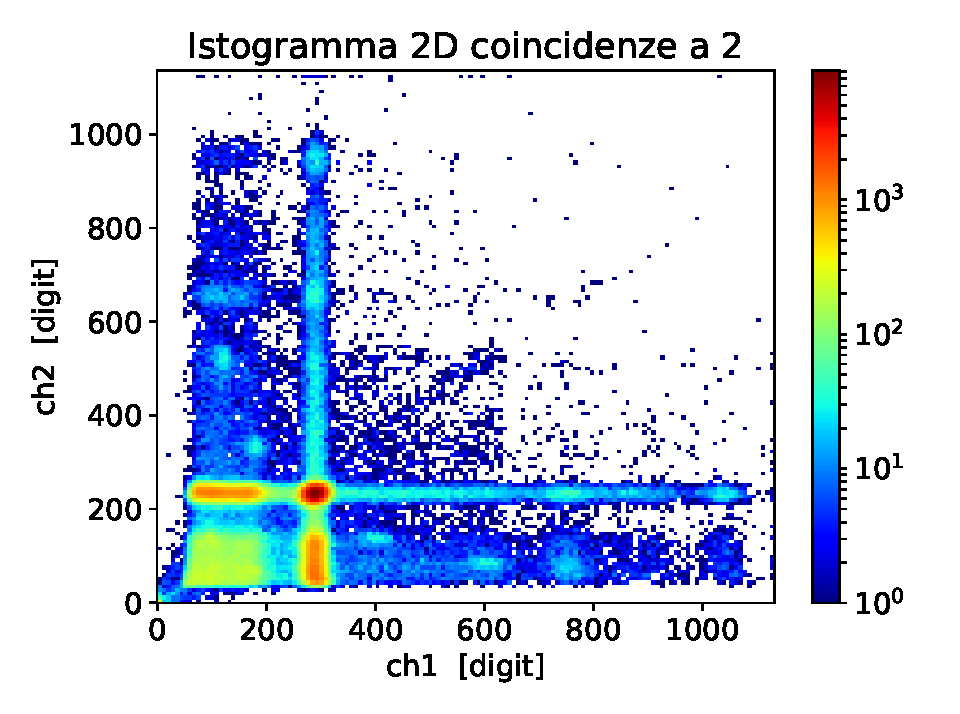
\includegraphics[width=\textwidth]{immagini/esempio}
\caption{Tipico istogramma 2D di una misura in coincidenza. La descrizione di questo grafico è presente nel testo.}
\label{scatter}
\end{figure}

Si vedono degli eccessi in alcuni punti del grafico che chiameremo in seguito \emph{strutture}. La più vistosa si manifesta quando entrambi i fotoni di annichilazione effettuano un processo fotoelettrico all'interno degli scintillatori. In basso a sinistra si nota invece la zona in cui entrambi hanno subito una diffusione Compton. Le bande arancioni intorno a questa zona rappresentano invece gli eventi in cui un fotone proveniente dall'annichilazione ha fatto fotoelettrico su un rivelatore e l'altro ha fatto Compton sull'altro.
La stessa cosa avviene con il fotone proveniente dal decadimento del neon, rappresentato dalle strutture nella parte centrale del grafico adiacente ai bordi della figura. La struttura più a destra (o più in alto) rappresenta l'arrivo simultaneo di un fotone di annichilazione insieme ad uno del neon. L'interpretazione degli eventi è analoga a quelli descritti precedentemente.
Le strutture non attese sono i due eccessi presenti nella zona in cui il fotone del neon e quello dell'annichilazione fanno entrambi scattering Compton. Queste strutture si manifestano a valori di energia coincidenti ai picchetti della spalla Compton.
\marginpar{``Picchetti della spalla Compton'', come aggiustarli?\\
\emph{La spalla Compton è la parte a destra,
il rialzo a sinistra viene chiamato backscattering in letteratura.
La frase che hai detto vuol dire semplicemente che se marginalizzi lo spettro 2D
i picchi rimangono visibili in quello 1D.}}

Per verificare la nostra ipotesi abbiamo messo i rivelatori nella configurazione di \autoref{spostati} sinistra, in modo da poterci aggiungere un mattone piombo come in \autoref{spostati} destra.
L'istogramma 2D corrispondente si trova in \autoref{spostato} sinistra: la struttura più popolata non è più data dalla rivelazione simultanea dell'annichilazione per effetto fotoelettrico, ma dalla somma degli eventi nelle bande che si incrociano.
\marginpar{Non è più la struttura più popolata.
Mi sa che non lo era neanche prima, era più \emph{densamente} popolata.
Identificarla con la configurazione dei fotoni.}
In questa configurazione non si nota più uno degli eccessi inattesi nominati prima: quello ad energia minore.
Adesso sono diventate evidenti due strutture circolari nella zona in basso a sinistra del grafico: esse e l'ultimo tipo di struttura rimasta scompaiono completamente quando effettuiamo la misura nella configurazione mostrata in \autoref{spostati} destra, come mostrato in \autoref{spostato} centro.
\marginpar{Nella caption di \autoref{spostato}:
le fasce in cui uno legge uno zero non si vedono più perché avevo zoomato il grafico.
Inoltre la spiegazione che sono il caso in cui uno legge uno zero non i pare esaustiva
perché, innanzitutto, non arrivano a 0.}

Alla luce di quanto osservato e analizzando i grafici, si trova che le strutture sopra descritte si presentano a coppie e la somma delle loro energie vale rispettivamente $m_e$, $2m_e$ ed $E_{\gamma}=\SI{1274}{keV}$.
Tali valori sono giustificati dal fatto che, in alcuni casi, un fotone rimbalza sul primo scintillatore su cui è arrivato e viene assorbito dall'altro. Se questo ha già assorbito l'altro fotone (possibile solo nell'annichilazione) la somma delle energie è proprio il doppio dell'energia del fotone singolo.

\begin{figure}[h]
\centering
\subfloat
{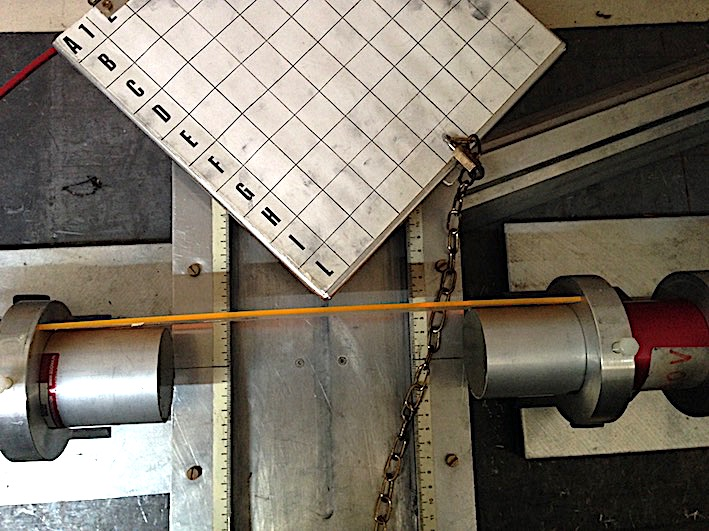
\includegraphics[width=0.49\textwidth]{immagini/alter}}
\hfill
\subfloat
{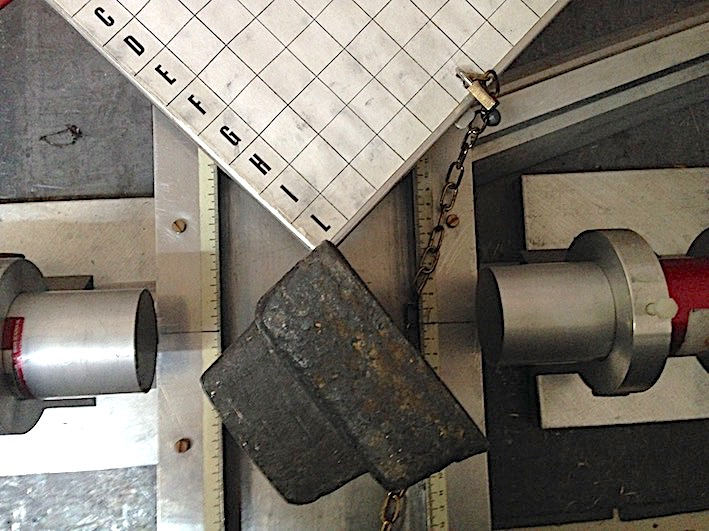
\includegraphics[width=0.49\textwidth]{immagini/spostati2}}
\caption{
A sinistra:
rivelatori posti uno di fronte all'altro senza schermatura.
La sorgente è nascosta nella casella L1 della scacchiera.
Il righello arancione serve per controllare che i due fotoni contrapposti di annichilazione
non possano raggiungere entrambi gli scintillatori.\\
A destra: aggiunta della schermatura di piombo per sopprimere i rimbalzi.}
\label{spostati}
\end{figure}

\begin{figure}[h]
	\hspace{-0.25\textwidth}
	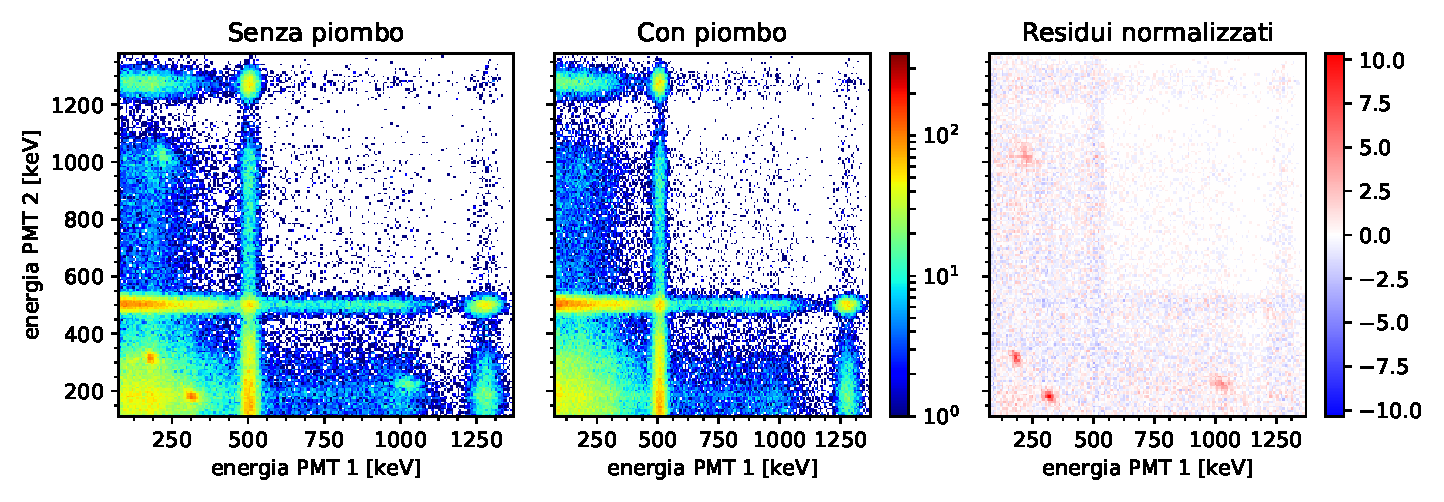
\includegraphics[width=1.5\textwidth]{immagini/diff}
	\caption{A sinistra: misura eseguita nella configurazione di \autoref{spostati} sinistra. \\
	Al centro: misura eseguita nella configurazione di \autoref{spostati} destra.  \\
	Le fasce densamente popolate adiacenti ai bordi della figura sono date dagli eventi in cui un rivelatore registra un evento mentre l'altro acquisisce uno zero.
	Una descrizione più dettagliata di questi grafici è presente nel testo.}
	\label{spostato}
\end{figure}

\subsubsection{Misura con un solo fotone}

Abbiamo effettuato la misura nella configurazione di \autoref{solo} sinistra e poi \autoref{solo} destra usando la sorgente di \cs{}: lo scopo della misura è evidenziare l'importanza dei rimbalzi tra scintillatori vicini.

\begin{figure}[h]
\centering
\subfloat
{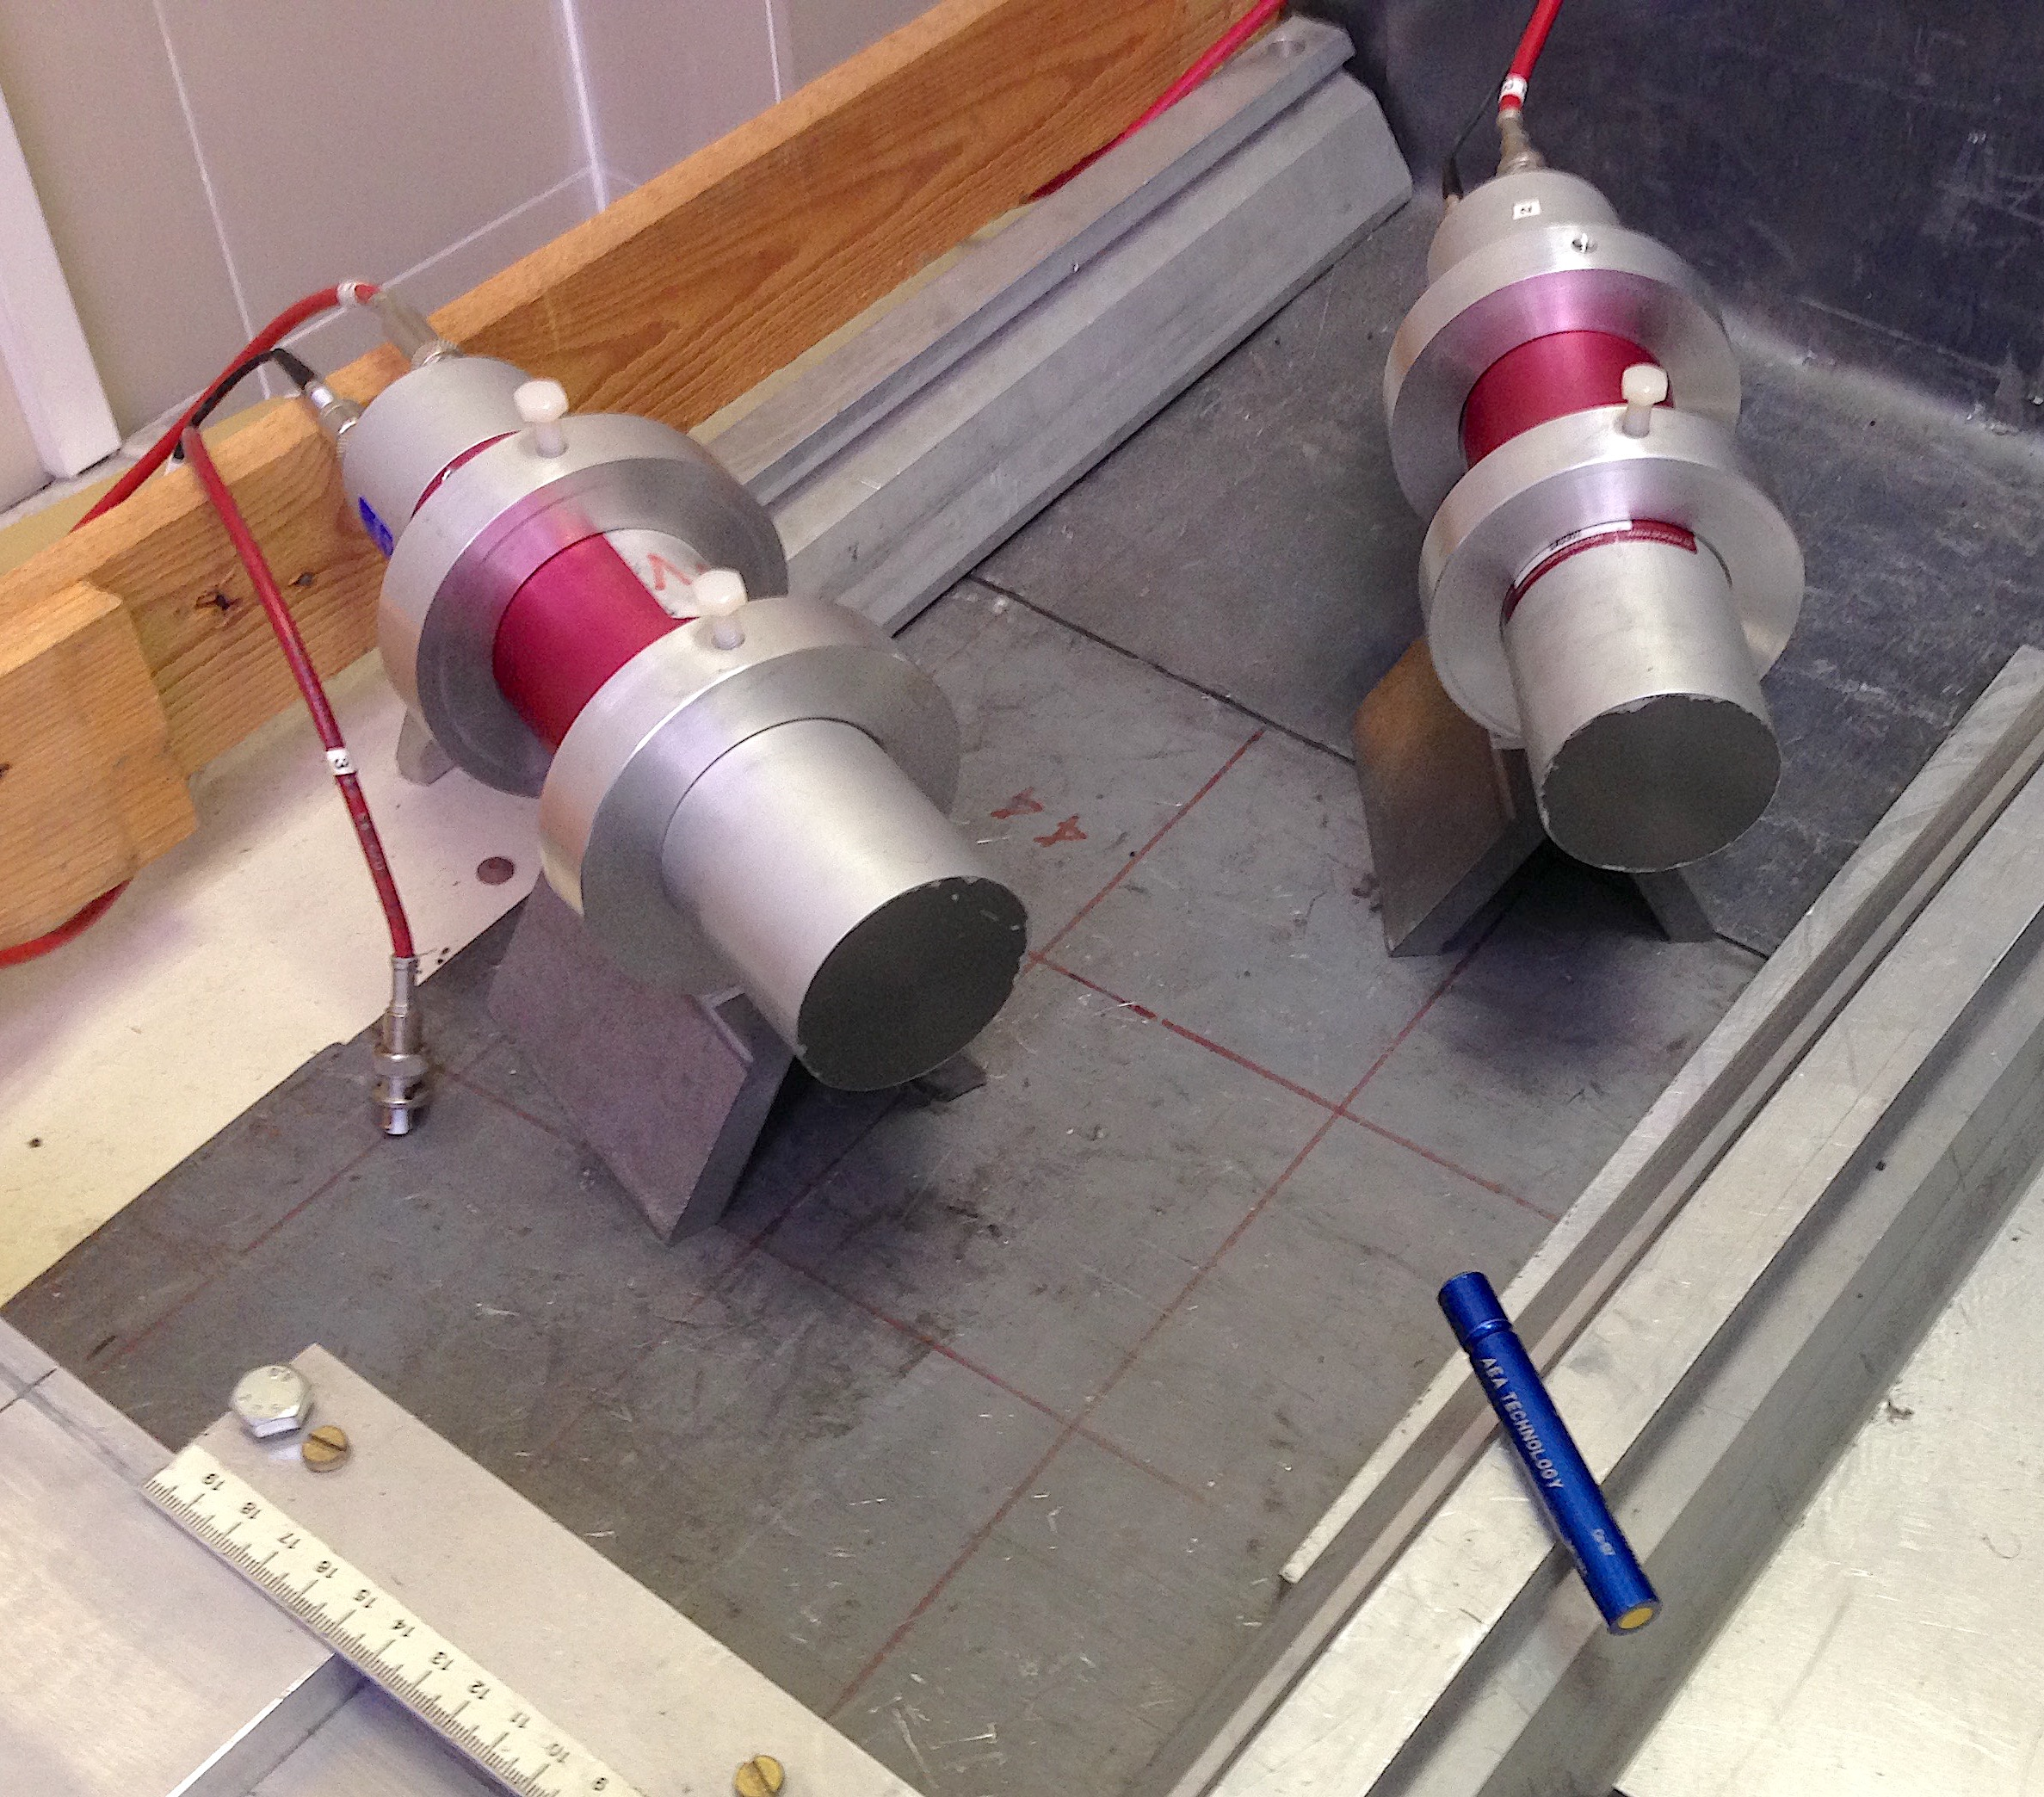
\includegraphics[width=0.49\textwidth]{immagini/rimb.jpg}}
\hfill
\subfloat
{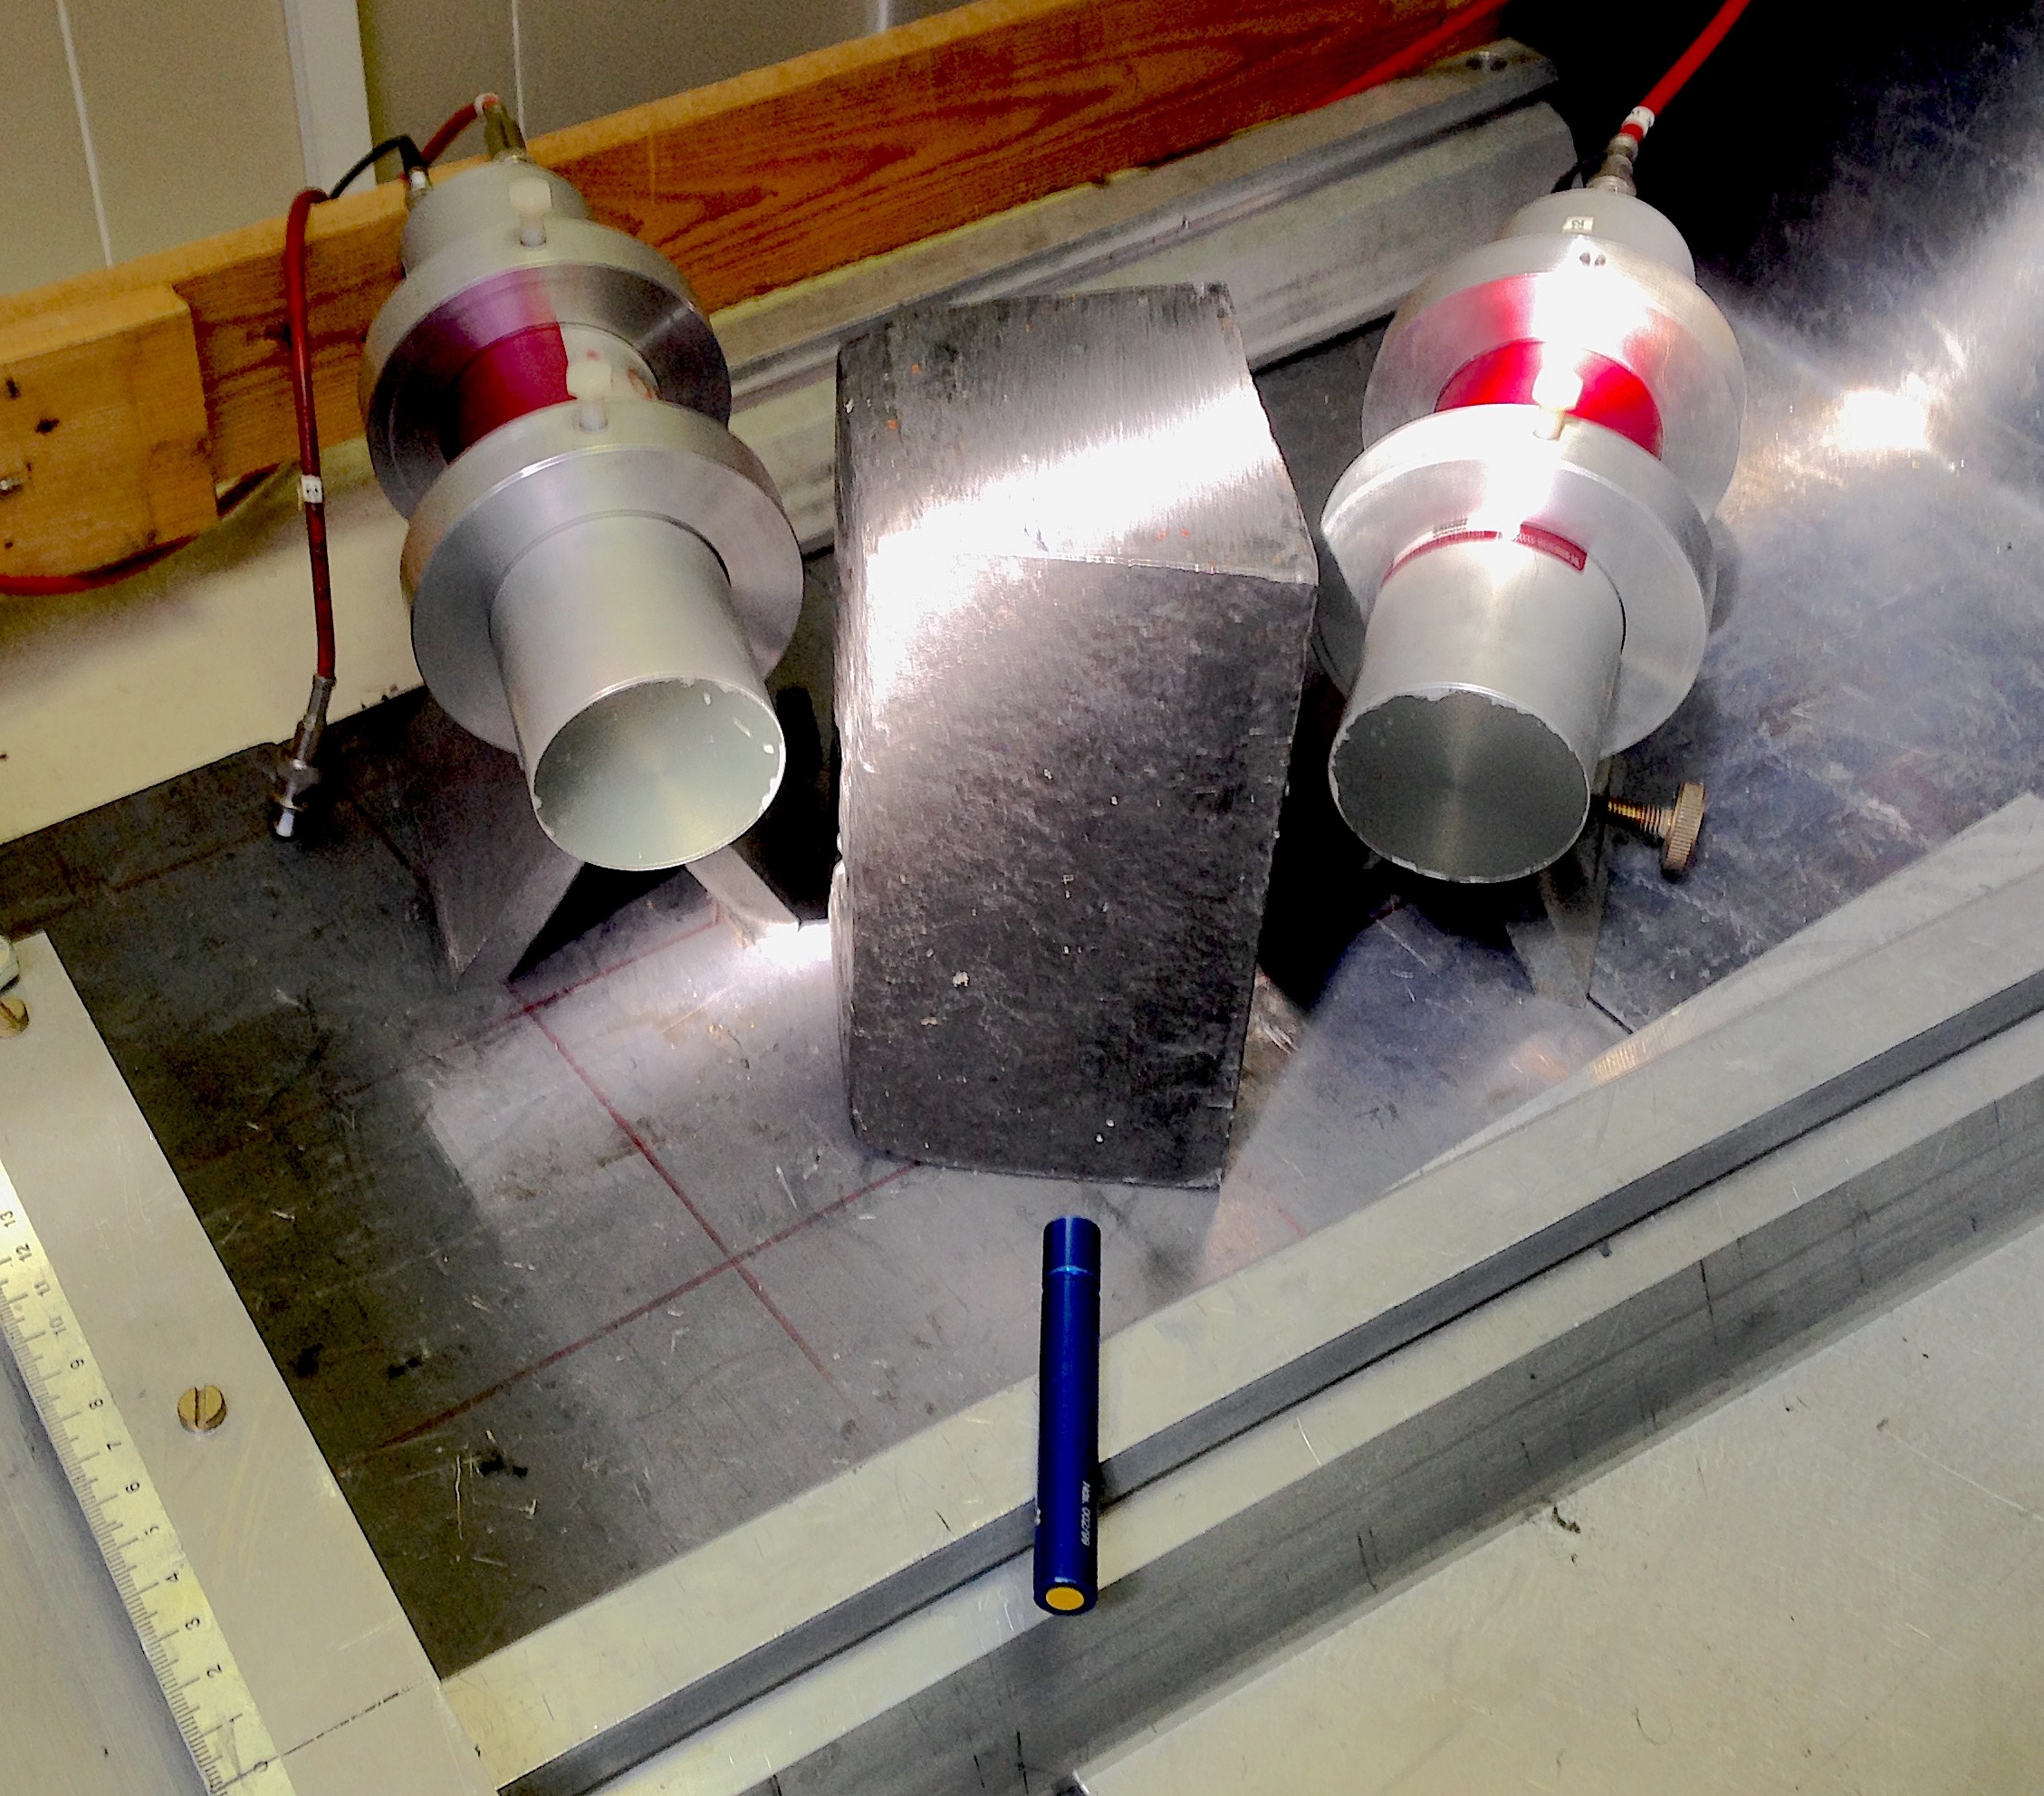
\includegraphics[width=0.49\textwidth]{immagini/norimb}}
\caption{\label{solo}
A sinistra:
configurazione usata per evidenziare la presenza di rimbalzi.
La sorgente è nel cilindretto blu.\\
A destra:
aggiunta del piombo che blocca i rimbalzi.}
\end{figure}

\begin{figure}[h]
\centering
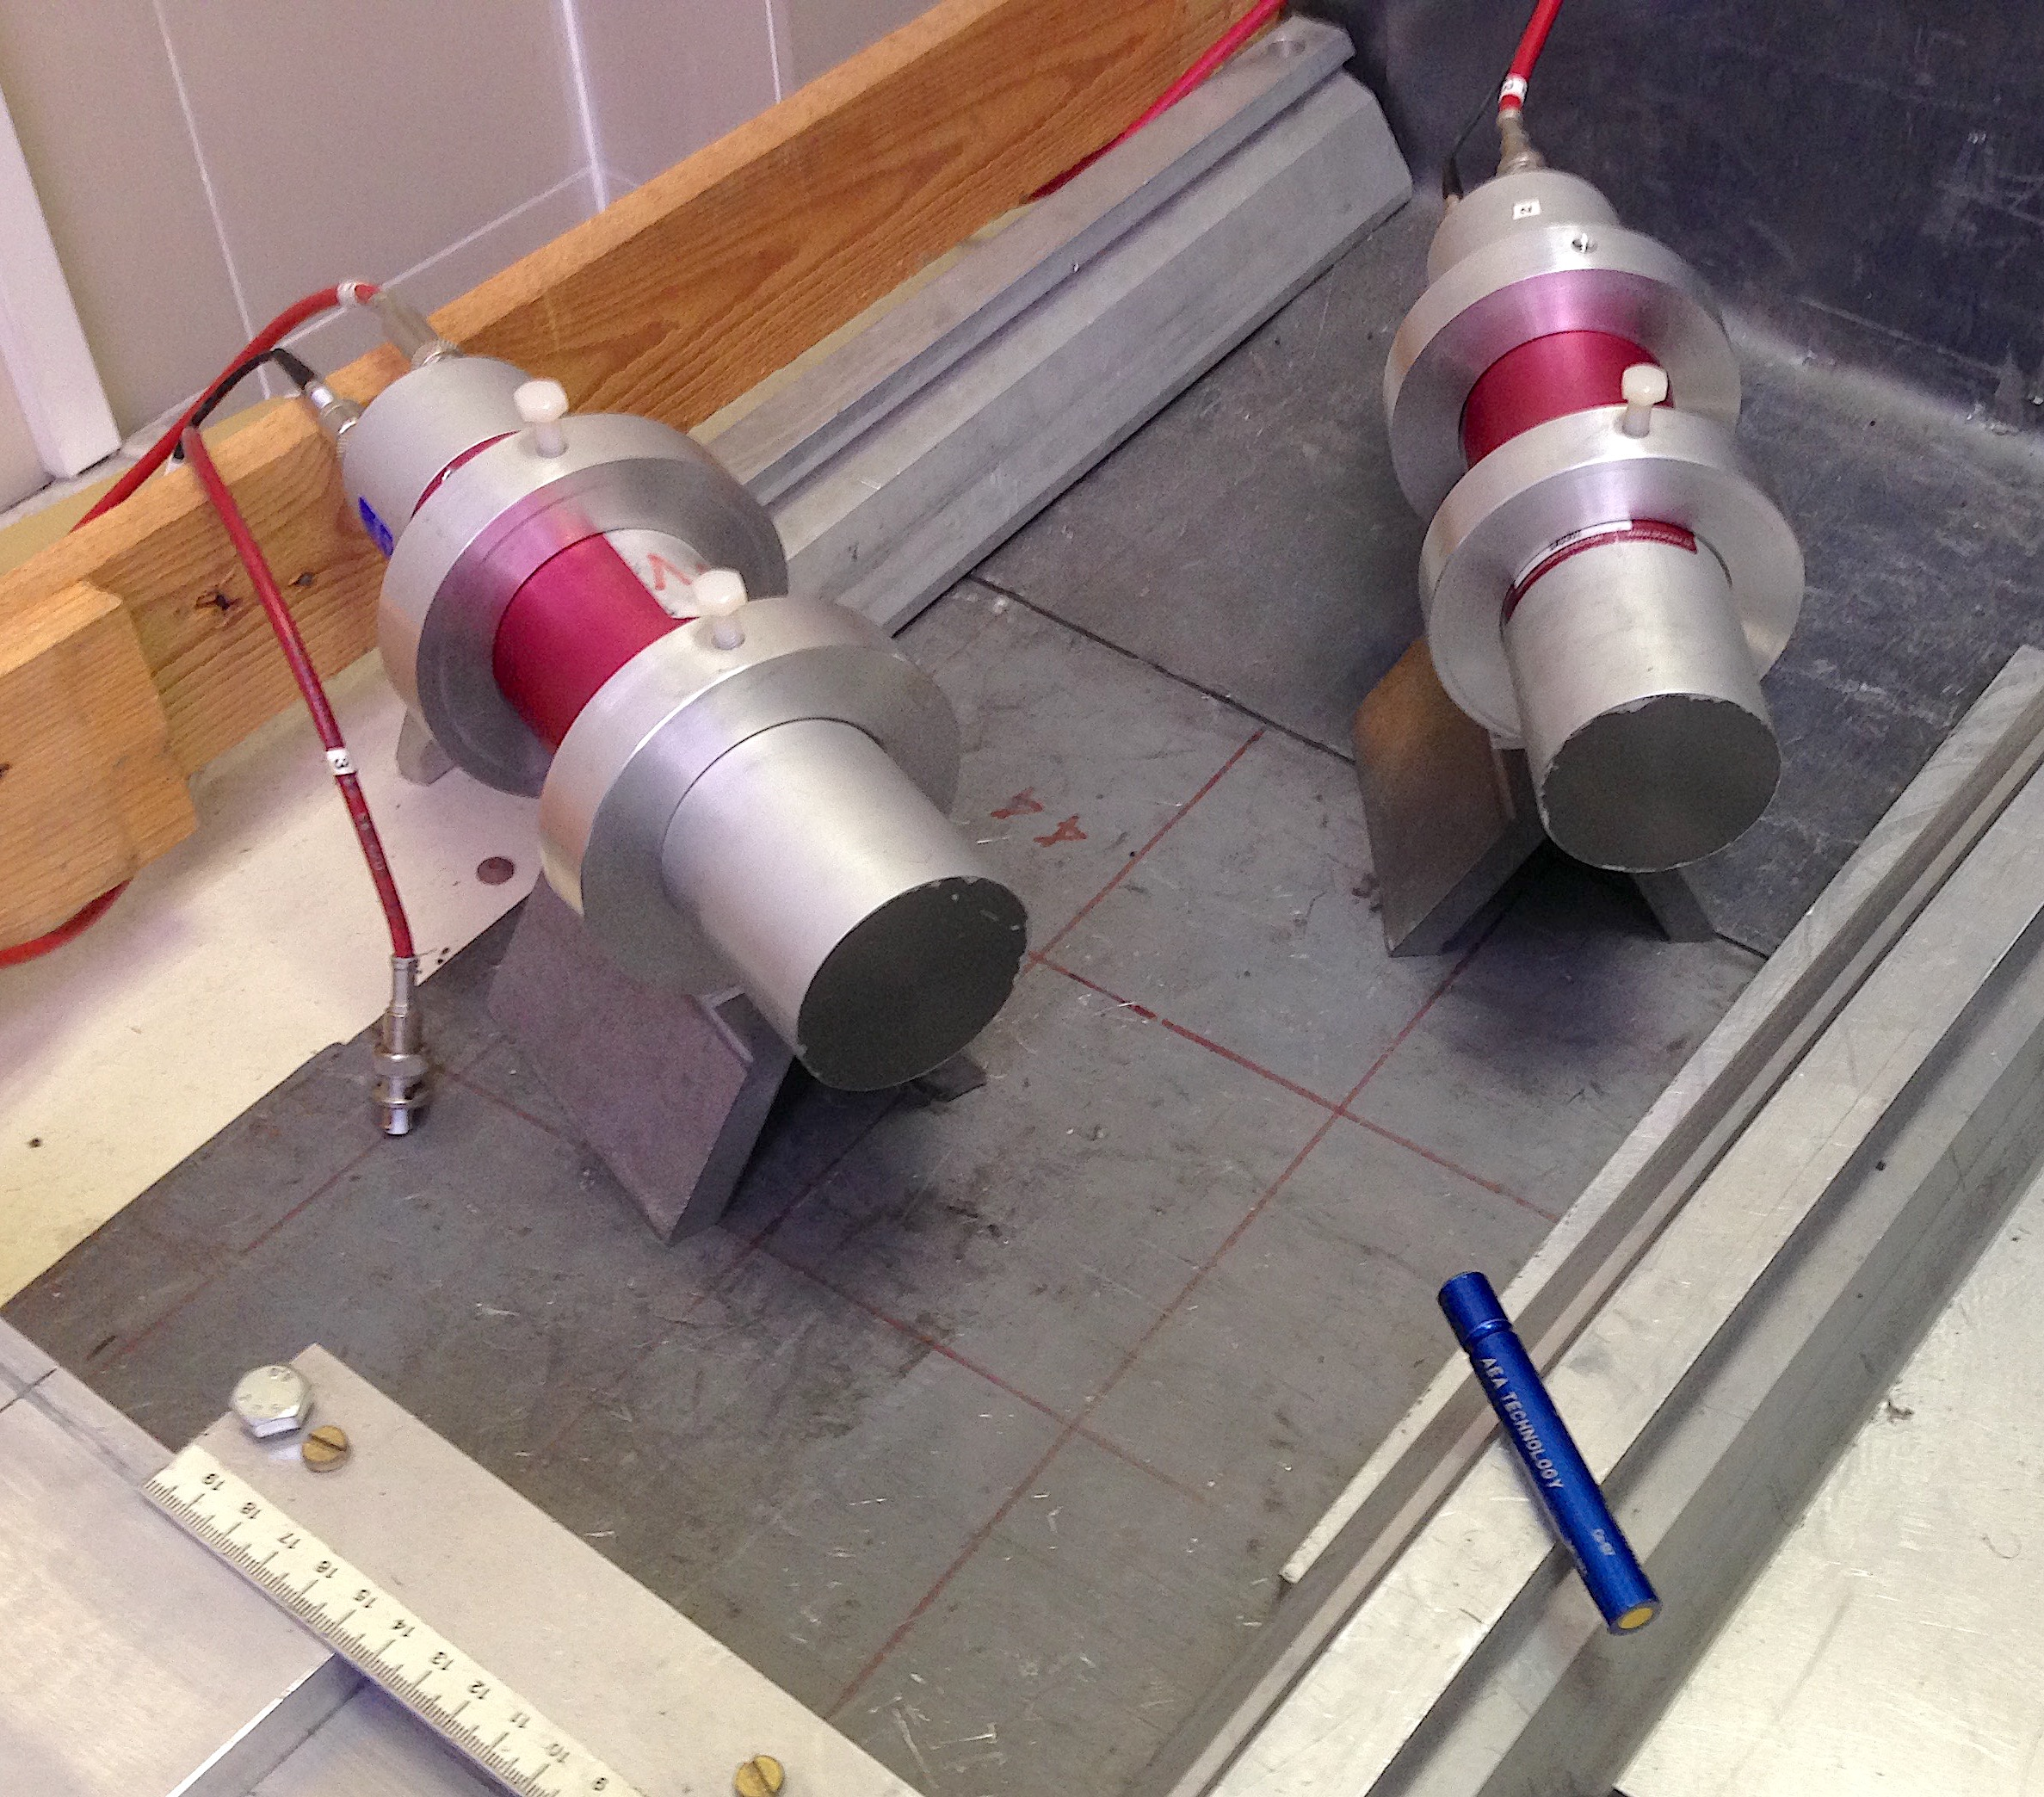
\includegraphics[width=\textwidth]{immagini/rimb}
\caption{\label{ce}
Spettro delle coincidenze tra i due scintillatori.
A sinistra: misura eseguita nella configurazione di \autoref{solo} sinistra.\\
A~destra: misura eseguita nella configurazione di \autoref{solo} destra.}
\end{figure}

L'istogramma 2D corrispondente alla \autoref{solo} sinistra è in \autoref{ce} sinistra: notiamo due accumuli proprio dove si trovavano in \autoref{spostato} sinistra. Anche questi scompaiono dopo aver aggiunto il piombo (\autoref{ce} destra). Gli eventi misurati possono essere coincidenze casuali oppure fotoni che hanno rimbalzato sul mattone o sulle pareti del contenitore in cui erano posizionati i rivelatori.
\marginpar{Ho cambiato la frase, ditemi se va bene.}

